\subsection{Protocol and independent controls}

All reported timings are completed local runs on the environment recorded
in the raw JSON, using Python 3.12.14. Measurements are not extrapolated
from operation counts. Mechanism-level counters are reported separately
from elapsed time. Historical source is frozen and hashed, and the
benchmark drivers verify that the relevant dependencies do not change
during a timing batch.

The two-meridian experiment uses twenty previously published diagrams,
with their original PDs and labels retained in a separate corpus file.
It performs nine shuffled measured rounds of five standalone variants:
baseline, a same-code baseline control, generation stamps alone, stamps
with candidate restriction, and the complete optimization. One warm-up
round is excluded. Whole-pipeline experiments use five rounds per diagram
in each of two option sets, comparing baseline, same-code control,
optimized stage, and the stage disabled. All existing filters, fallback
methods and time limits are retained. Reported paired speedups are
\emph{medians of within-round ratios}; they need not equal the ratio of
the two separately reported medians.

The incidence experiment uses twenty exact supplied interval systems:
five modulus bit lengths and four port counts, with three shuffled rounds.
An independent residue-endpoint formula checks every answer; literal
union--find also checks the eight small cases. The special formula is
cheaper on this intentionally structured family and is not presented as
an algorithm being beaten by the generic engine.

The normal-surface experiment measures full aggregate topology, proof
production and independent replay separately. Small explicit polygon
and Regina component controls check overlapping topology outputs; they
also return individual coordinate records and do not implement the same
proof protocol. They are appropriate independent controls, not identical
whole-workflow baselines. The complete raw normal benchmark includes
the input vector for every measured row.

\subsection{Correctness evidence}

The interval producer and independent verifier passed 26 focused test
methods. The producer tests include exhaustive pairs of isometries on
universes of size at most four, 4,000 seeded arbitrary systems, inverses
and reflected-coordinate invariance, support-hull and adjacent-period
regressions, and 12,001-bit widths. A separate development audit compared
40,000 arbitrary systems with a finite disjoint-set oracle and replayed
10,000 generated certificates. The reproducible focused suite is retained;
those larger development totals are not added to the count of test methods.

Ten incidence test methods include 180 randomized literal histograms,
every marked-subset identity on those cases, duplicate and empty ports,
huge integers, forged proofs, and the guarantee that replay does not
invoke the producer. Eight tests cover the imported normal extractor and
eight new tests cover native topology, disc essentiality, coning,
hexadecimal proof transport, malformed inputs and cancellation.

The strengthened normal geometry audit has the following completed scope:
\begin{center}
\begin{tabular}{@{}lr@{}}
\toprule Check & Count\\\midrule
Geometric input vectors & 1,561\\
Native Regina input vectors & 799\\
Component records compared & 15,978\\
Closed component records & 290\\
Nonorientable component records & 108\\
Inputs mixing closed and boundary-bearing components & 8\\
Independently replayed topology certificates & 2,360\\
Malformed-input, altered-proof and interruption checks & 17\\\bottomrule
\end{tabular}
\end{center}
The native audit includes vertex normal surfaces and compatible sums in
balls, spheres, lens spaces, products, a solid Klein bottle, the three-torus,
and layered solid tori. It compares against native component vectors,
Euler characteristic, orientation and boundary counts. An additional
independent check uses Regina's ambient edge classes for $V$, derives $E$
from native Euler characteristic, checks boundary arc counts, and tests
the boundary parity class using Gaussian elimination over $\F$ rather
than our signed disjoint-set structure and graph traversal.

The two-meridian changes pass fourteen targeted methods, including the
eight previous methods unchanged. New exhaustive checks cover all 4,096
four-arc systems built from distinct-arc crossing types, all 512 three-arc
systems including productive unary rules, and 400 random degenerate
systems. Repeated fixed-point closure and the frozen old queue routine
serve as separate oracles. Candidate completeness, proper-closed-set
pruning, first successful pair, exact derivation order, resource behavior,
and replay without search are checked. All twenty natural fixtures have
the same exhaustive outcomes and byte-identical positive certificates.

The complete maintained test suite, including the new modules and imported
extractor tests, passes: \textbf{833 tests in 122.148 seconds}. The full log
is delivered. This result followed the worker repair described below; the
initial failing run is retained as separate evidence.


\subsection{Seed-search results on natural diagrams}

\begingroup\small\setlength{\LTpre}{6pt}\setlength{\LTpost}{6pt}
\begin{longtable}{@{}lrrrrrr@{}}
\toprule Diagram & $n$ & Old trials & New trials & Old ms & New ms & Paired ratio\\\midrule\endhead
survivor-00 & 16 & 60 & 23 & 0.873 & 0.593 & 1.319\\
survivor-01 & 15 & 120 & 23 & 0.882 & 0.295 & 3.001\\
survivor-02 & 15 & 16 & 16 & 0.541 & 0.546 & 1.071\\
survivor-03 & 13 & 14 & 14 & 0.453 & 0.421 & 1.037\\
mirror-03 & 13 & 14 & 14 & 0.422 & 0.421 & 1.015\\
survivor-04 & 13 & 14 & 14 & 0.424 & 0.418 & 1.009\\
survivor-05 & 13 & 14 & 14 & 0.619 & 0.464 & 1.368\\
survivor-06 & 12 & 21 & 14 & 0.499 & 0.463 & 0.965\\
survivor-07 & 12 & 28 & 15 & 0.489 & 0.423 & 1.157\\
survivor-08 & 11 & 12 & 12 & 0.355 & 0.346 & 1.021\\
mirror-08 & 11 & 12 & 12 & 0.533 & 0.534 & 1.012\\
survivor-09 & 11 & 12 & 12 & 0.366 & 0.344 & 1.053\\
survivor-10 & 11 & 12 & 12 & 0.351 & 0.351 & 0.994\\
survivor-11 & 11 & 14 & 13 & 0.476 & 0.553 & 0.918\\
Gordian & 141 & 10,011 & 274 & 297.346 & 3.460 & 85.861\\
Trefoil & 3 & 4 & 4 & 0.112 & 0.118 & 0.951\\
Figure-eight & 4 & 5 & 5 & 0.136 & 0.143 & 0.942\\
Hard unknot 8 & 8 & 9 & 9 & 0.257 & 0.271 & 0.987\\
Conway & 11 & 66 & 19 & 0.438 & 0.236 & 1.790\\
Kinoshita--Terasaka & 11 & 66 & 19 & 0.449 & 0.238 & 2.028\\
\bottomrule\end{longtable}\endgroup


The largest difference is on Gordian's 141-crossing diagram. The baseline
examines 10,011 seed sets, uses 4,347,002 work units, and takes a median
297.346 milliseconds. The optimized query examines 274 seed sets, uses
12,251 work units, and takes 3.460 milliseconds. The median matched ratio
is 85.861, while the baseline-versus-identical-control ratio is 0.991.
There are 274 candidate edges before closed-set pruning. The latter
excludes 141 later edges, so the executed trials comprise 141 singletons
and 133 pairs. The largest proper closure has five arcs.

Every one of the 900 measured standalone calls completes its exhaustive
class query. Sixteen fixtures receive a conclusive knot verdict with
the exact frozen positive certificate. Gordian, survivor-01, Conway and
Kinoshita--Terasaka instead exhaust the two-seed derivation class and
return \code{INCONCLUSIVE} for knot type. The previously capped Gordian
query failed to exhaust its candidate list; the new query completes far
below the same two-million-unit allowance. This is a capacity improvement
for the class test, not an independent Gordian unknot certificate.

The mechanism ablation on Gordian separates the gains:
\begin{center}
\begin{tabular}{@{}lr@{}}
\toprule Standalone variant & Median milliseconds\\\midrule
Original dense preparation & 297.346\\
Generation arrays only & 27.577\\
Generation arrays and first-firing candidates & 3.587\\
Complete change, including proper-closure pruning & 3.460\\\bottomrule
\end{tabular}
\end{center}
\begin{figure}[ht]
\centering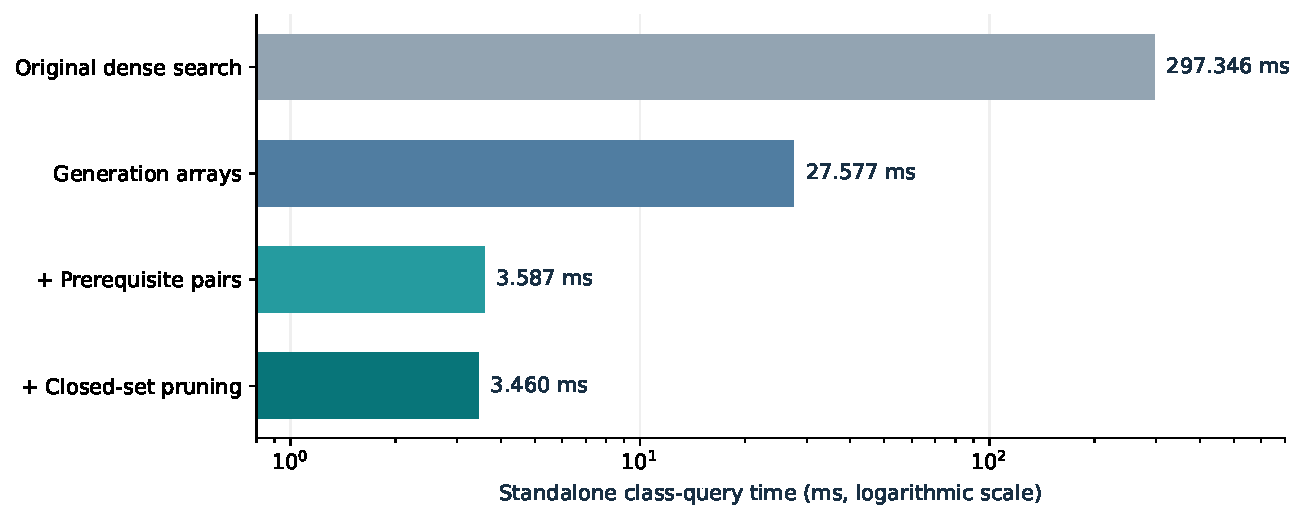
\includegraphics[width=.94\textwidth]{figures/seed_ablation.pdf}
\caption{Measured Gordian two-seed class query. The logarithmic horizontal
scale separates the reusable-state gain from the candidate-set theorem.
This figure does not report whole-knot recognition time.}
\end{figure}

\subsection{Whole-pipeline results and negative cases}

The 800 measured whole-pipeline calls contain 780 completed verdicts,
all equal to the established corpus label, and twenty censored ordinary
Gordian calls that return \code{UNKNOWN}. A timeout is not assigned an
artificial finite speedup.

For survivor-00, the ordinary option set has baseline and new medians
1.950 and 1.690 milliseconds and a median matched speedup of 1.221.
With compressed group search enabled, the corresponding medians are
1.968 and 1.580 milliseconds and the matched speedup is 1.245.

For Gordian with compressed group search, the matched ratio is only
1.034; the separately measured medians are 1.338 seconds for the baseline
and 1.375 seconds for the changed version. Their different ordering is
possible because the median of ratios and the ratio of medians are
different statistics. It illustrates why this small whole-query change
must not be described as a robust universal speedup. The subsequent
roughly 1.3-second recognizer dominates the saved seed work. The ordinary
Gordian configuration never finishes within its cap in either version.

Several small standalone cases regress, including trefoil, figure-eight
and survivor-11; the complete table and A/A controls retain those results.
The stage remains opt-in. The measurements support an exact search
improvement with a large local gain on sparse failures, not a blanket
improvement on every recognized knot.

\subsection{Native compressed surface scaling}
The layered-solid-torus family is inherited from the preceding reports.
Its supplied meridian vector has Fibonacci growth; no claim of a new family is made.
Each measured vector is certified as one orientable disc with one essential boundary circle.
The following timings use three shuffled rounds, with raw samples retained.
\begin{center}\small\begin{tabular}{@{}rrrrrr@{}}
\toprule $t$ & Disc-count bits & Count ms & Proof ms & Replay ms & Proof KiB\\\midrule
1 & 2 & 0.368 & 0.365 & 0.316 & 3.7\\
4 & 5 & 3.564 & 3.951 & 1.585 & 29.8\\
8 & 8 & 12.886 & 13.315 & 3.783 & 87.8\\
12 & 11 & 29.744 & 30.479 & 7.281 & 169.1\\
16 & 14 & 80.155 & 82.503 & 18.313 & 274.1\\
32 & 25 & 225.174 & 265.364 & 34.092 & 938.4\\
64 & 47 & 1310.748 & 1516.839 & 188.950 & 3446.5\\
128 & 92 & 8045.830 & 8103.743 & 628.618 & 13188.4\\
\bottomrule\end{tabular}\end{center}
At $t=128$, the input has 384 nonempty stacks, 764 surface face bands, and
\[N=2\,791\,715\,456\,571\,051\,233\,611\,642\,548\]
normal discs. The ordinary orbit query needs 390 cycles and 41,643 transmissions;
its orientation lift needs 779 cycles. These are algorithmic counts, not sheet counts.
The full five-query certificate occupies 13,504,926 bytes as compact JSON.
The size is charged explicitly; binary geometry does not make certificate transport free.

\begin{figure}[ht]\centering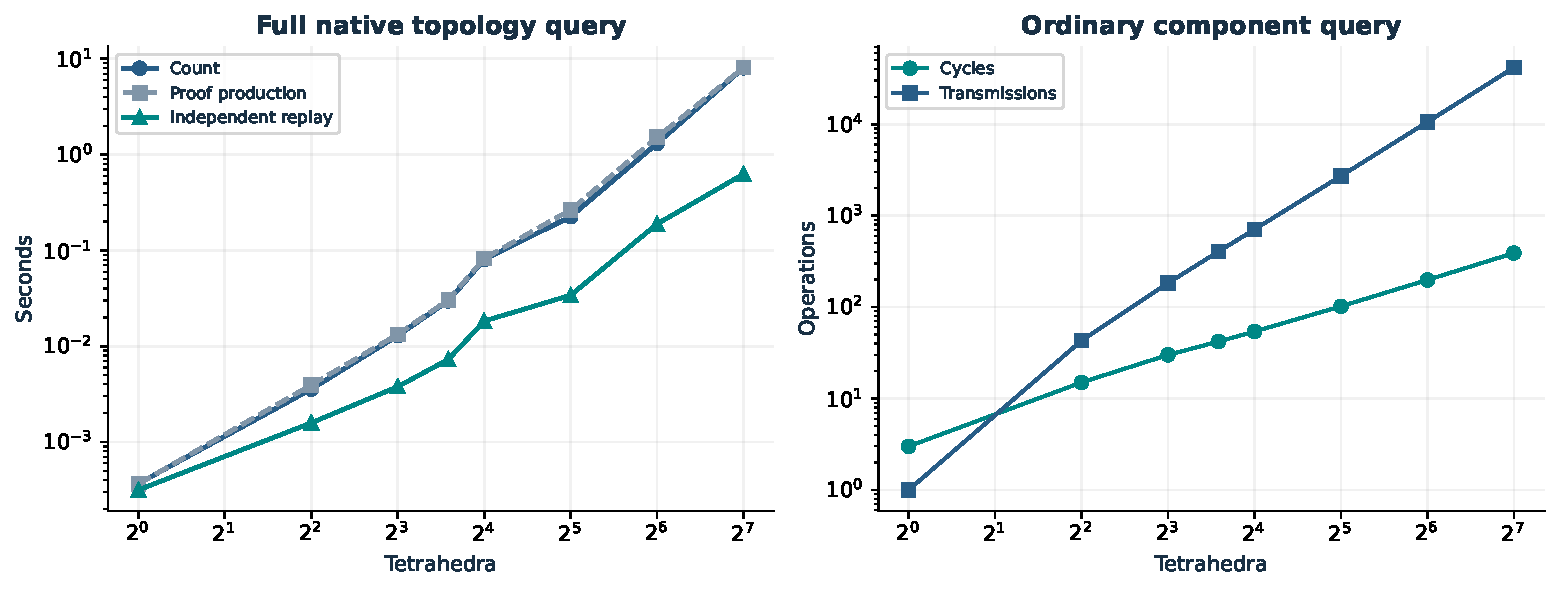
\includegraphics[width=\textwidth]{figures/normal_scaling.pdf}
\caption{Measured native topology costs and ordinary orbit work on supplied Fibonacci
meridian vectors. Lines join measured points only. They are not a fitted universal
complexity law.}\end{figure}

The small explicit controls are often faster. At $t=12$, literal polygon assembly
takes 9.659 ms versus 29.744 ms for the new aggregate query; Regina's component
routine takes 0.906 ms. At $t=16$, the literal control takes 98.205 ms versus
80.155 ms, while Regina remains faster at 3.226 ms. Those controls return a
different output protocol, and these figures are not claimed as certificate-level speedups.
Both explicit controls are restricted to at most 20,000 discs in the final benchmark.
Regina's documented \code{components()} routine explicitly constructs normal discs
\cite{reginadoc}; an initial uncapped diagnostic reached the 64-tetrahedron case
and raised \code{MemoryError: std::bad\_alloc}. Its aborted log is retained separately
and contributes no primary timing ratio. We then applied the same finite-oracle
cap to both explicit controls and reran the complete source-guarded benchmark.
The large rows therefore establish native compressed completion and proof replay,
not a fabricated ratio against a censored explicit computation.


\subsection{Port-incidence costs and the output contract}

For the family $N=7\cdot2^{4096}$, the primary pairings identify residues
modulo $2^{4096}$ and the selected ports are supplied unions of intervals.
The measured medians are:
\begin{center}
\begin{tabular}{@{}rrrrr@{}}
\toprule Ports & Histogram slots & Count (ms) & Proof (ms) & Replay (ms)\\\midrule
2 & 4 & 0.232 & 0.253 & 0.214\\
4 & 16 & 1.761 & 1.625 & 1.313\\
6 & 64 & 8.867 & 9.911 & 7.780\\
8 & 256 & 48.168 & 54.247 & 40.698\\\bottomrule
\end{tabular}
\end{center}
The eight-port proof serializes to 13,866,578 bytes in compact JSON.
This cost is recorded and charged even though the mathematical output
has only 256 integer slots. Only the selected 1,024-bit four-port proof
is retained as a separate replay fixture; the larger proof's size and
digest are in the data. Count-only mode does not retain those traces.

The small-universe comparison supplies an important counterweight. For
$N=7\cdot2^{12}$ and eight ports, the new method takes 25.059 milliseconds
versus 10.355 milliseconds for literal enumeration. With two ports at the
same size, it takes 0.151 milliseconds versus 8.517 milliseconds. Avoiding
sheet expansion does not automatically win when the expanded instance
is small and the number of coned queries is large.

These are generic queries on supplied interval systems. They are not
whole-recognizer timings, not a benchmark against the weighted AHT
algorithm, and not evidence that all geometric attachment information
has been recovered.

\subsection{An inherited worker failure repaired separately}

The first full regression run executed 833 tests and reproduced one
existing failure in the optional normal-surface subprocess wrapper. A
500,000-character request was not completely transmitted when a timed
\code{communicate} call was retried with no input on this Python version.
This defect predates the interval and seed changes and had already been
identified in incoming reports; the maintained baseline still contained
the failing path.

The focused repair gives one worker thread ownership of a single
\code{communicate(payload)} call while the main thread polls its future
for cancellation and deadline handling. On exit the child is killed
when necessary, reaped, the communication owner is joined, and the pipes
are closed. The existing eight worker tests pass, including delayed
large-input transmission, local timeout, global cancellation, and
actual Regina verdicts. This is an engineering repair, not one of the
mathematical advances. The seed benchmark does not import this worker
path, so its measured dependency hashes remain unchanged.

\subsection{Interpretation of the evidence}

The strongest experimental conclusion is agreement across independent
representations, coupled with successful processing of genuine normal
vectors whose disc multiplicity is far beyond enumeration. The strongest
search improvement is the reduction from a quadratic candidate set to
a linear one under a checked hypothesis, combined with output-sensitive
closure work. The data show where each matters and where it does not.
None of the experiments estimates a universal hierarchy depth or proves
the missing complete recognition bound.
